%%%
% Tech report template. Compile with pdflatex
%%%
%\documentclass[pdftext,twoside,12pt]{report}
\documentclass[pdftext,twoside,11pt]{article}

\usepackage[a4paper,lmargin=2.5cm,rmargin=2cm,tmargin=1cm,bmargin=1cm,includehead,includefoot]{geometry}
\usepackage[german,english]{babel}
\usepackage{url}
\usepackage{subfig}
\usepackage{fancyhdr}
\usepackage{caption}
\usepackage{array}
\usepackage{amsmath} % needed for subequations
\usepackage{amssymb}
\usepackage{marvosym} % for the Euro symbol
\usepackage{mathptmx}
\usepackage{multirow}
\usepackage[small,compact]{titlesec}  %for compressed Section titles
\usepackage{mdwlist}  %for compressed itemized lists
\usepackage{setspace} %for chaging spacing in environments (see biblio)
\usepackage[numbers,sort&compress]{natbib}
\usepackage[scaled=.90]{helvet}
\usepackage{times}
\usepackage[T1]{fontenc}
%\usepackage[latin1]{inputenc}
\usepackage[utf8]{inputenc}
\usepackage{graphicx} 
\usepackage{pgf}
\usepackage{hypernat}
\usepackage{hyperref}

%%% Package options %%%

\hypersetup{colorlinks=true, breaklinks=true, pagebackref=true,
  urlcolor=blue, linkcolor=blue,anchorcolor=blue,citecolor=blue,
  pdfpagemode = UseNone, %FullScreen, %UseThumbs, %UseOutlines,
  pdfauthor = {},
  pdftitle = {},   
  pdfsubject = {},
  pdfkeywords = {}
}

\DeclareGraphicsExtensions{.jpg,.pdf,.mps,.png}
\graphicspath{{img/} {./}} %put all figures in these dirs

\urlstyle{rm} %so it doesn't use a typewriter font for urls.

%\newcommand{\bibfont}{\scriptsize} %for smaller fonts in biblio

\renewcommand{\captionfont}{\small \sffamily}

\renewcommand\floatpagefraction{.9}
\renewcommand\topfraction{.9}
\renewcommand\bottomfraction{.9}
\renewcommand\textfraction{.1}   

\setlength{\bibsep}{1pt}           %for compressed itemized list on biblio
\setlength{\topsep}{0pt}
\setlength{\itemsep}{0pt}
\setlength{\partopsep}{0pt}
\setcounter{totalnumber}{50}
\setcounter{topnumber}{50}
\setcounter{bottomnumber}{50}

%Example of image declaration (declared once in pdf file, reduces file size)
%\pgfdeclareimage[height=0.8cm]{logo}{img/logo} 
%Use with:
%\pgfuseimage{logo}

% Headers and Footers
\pagestyle{fancy}
\fancyhead{} % reset headers
\fancyfoot{} % reset footers
\fancyhead[LO]{\textsf{\textbf{TITLE}}}
\fancyhead[CO]{\date{\today}}
\fancyhead[RO]{AUTHOR}
% remove horizontal lines between text and headers and footers
\renewcommand{\footrulewidth}{0pt}
\renewcommand{\headrulewidth}{0pt}


%  Title page
\title{A Review of Recent Research in Extracting Information From Medical Textual Documents}
\author{AUTHOR\\
  University of Florida\\
}
\date{\today}


\begin{document}

%\thispagestyle{empty}
\maketitle

% keywords

% Use with {report} documentclass
% \chapter{The beginning}
% \label{cha:beginning}

%----------------------------------------------------------%
\section{Automated identification of extreme-risk events in clinical incident reports, JAMIA 2012}
\label{sec:intro} 
\begin{itemize}
\item Objectives: classification problem
\item Methods: Naive Bayes and Support Vector Machine. 
\item Result assessments: precision,recall,F-measure,AUC.
\item Feature extraction:  Punctuation removed, converted to lower case,'bags of words'
\item Input representation: binary,term-frequency, thresholding,tf-idf
\item Feature selection: excluding words in similar frequency(dimensionality reduction)
                              excluding determiners, prepositions, pronouns, conjunctions(pos tagging)
                              stemming, bigrams.
\item Training and validating the classifiers: Naive Bayes, SVM(linear,Polynomial,RBF), 10-fold cross-validation.
\end{itemize}
\section{Extracting Information from Textual Documents
 in the Electronic Health Record:A Review of Recent Research.}
\label{sec:intro} 
\begin{itemize}
\item Spell checking, word sense disambiguation(?), POS, Contextual features like negation, temporarily, and subject identification.

\item Automatic de-identification uses the extraction of personal information before its removal. Rule-based NER.
\item Contextual Feature Detection and Analysis.
             Negation(e.g. “denies any chest pain”) temporarily(e.g. “fracture of the tibia 2 years ago”). Event subject identification(e.g. “his mother has diabetes”). 
                          NegExpanding,NegEx,Negfinder: a program detecting negation terms 
                          TimeText detected temporal relations. 
\end{itemize}

\section{Automated systems to identify relevant
documents in product risk management}
\label{sec:intro} 
\begin{itemize}
\item  logistic regression, K-nearest neighbour, Naive Bayes, SVM
\item  Word occurrence, Binary frequence, TF-IDF. 
\item  stemming, remove prepositions, indentify acronums, synonyms obtained from Omniviz.
\end{itemize}
\section{De-Indentification}
\label{sec:intro} 
\begin{itemize}
\item  Patient's and doctor's first and last names 
\item  Id numbers, Phone, fax, pager numbers, Hospital names, Geographic locations, Dates, Ages above 90 
\end{itemize}
features of the text used in de-identification
\begin{itemize}
\item Target word to be classified
\item Words up to 2 words left/right of target
\item Target part of speech
\item Target capitalization
\item Target length and others.  
\end{itemize}

\section{WordNet, UMLS, MetaMap}
\label{sec:intro} 
\begin{itemize}
\item WordNet® is a large lexical database of English. Nouns, verbs, adjectives and adverbs are grouped into sets of cognitive synonyms (synsets), each expressing a distinct concept. Synsets are interlinked by means of conceptual-semantic and lexical relations.WordNet's structure makes it a useful tool for computational linguistics and natural language processing.
\item The UMLS project is an effort to overcome two significant
 barriers to effective retrieval of machine-readable information.
       The first is the variety of ways the same concepts are expressed
      in different machine-readable sources and by different people. disparate databases and systems.

\item MetaMap is a highly configurable program developed by the National Library of Medicine (NLM) to map biomedical
 text to the UMLS Metathesaurus or, equivalently, to discover Metathesaurus concepts referred to in text. 
MetaMap uses a knowledge-intensive approach based on symbolic, natural-language processing (NLP) and 
computational-linguistic techniques. Besides being applied for both IR and data-mining applications, 
MetaMap is one of the foundations of NLM's Medical Text Indexer (MTI) which is being used for both 
semiautomatic and fully automatic indexing of biomedical literature at NLM. 
\end{itemize}

\section{Coreference resolution: A review of general methodologies and applications
in the clinical domain, Journal of Biomedical Informatics, 2011}
\label{sec:intro} 
\begin{itemize}
\item  extract drug names and signatures. extract principal diagnosis from discharge summary.
       smoking status and medication dosage, frequency, and route.
\item
\begin{center}
  %\begin{multicols}{2}
      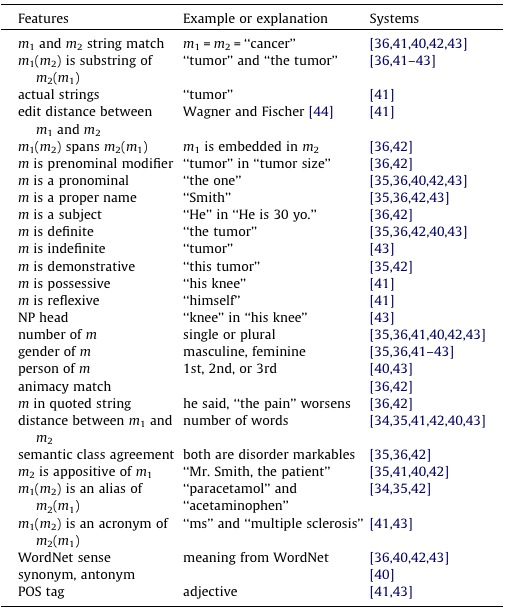
\includegraphics[height=30em,width=20em]{feature.jpg}
      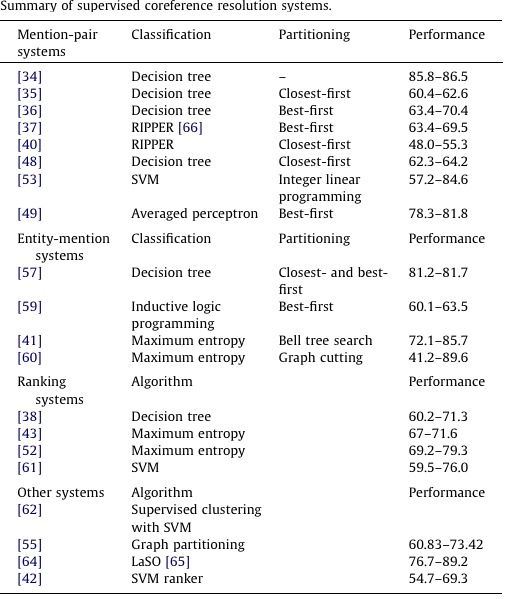
\includegraphics[height=30em,width=20em]{comparision.jpg}
  %\end{multicols}
\end{center}

\item   combined with Andrew MacCallum's most recent work, UMLS,MetaMap,and our system? 
\end{itemize}

\section{Lexical patterns, features and knowledge resources for coreference resolution
in clinical notes, Journal of Biomedical Informatics, 2012}
\label{sec:intro} 
\begin{center}
  %\begin{multicols}{2}
      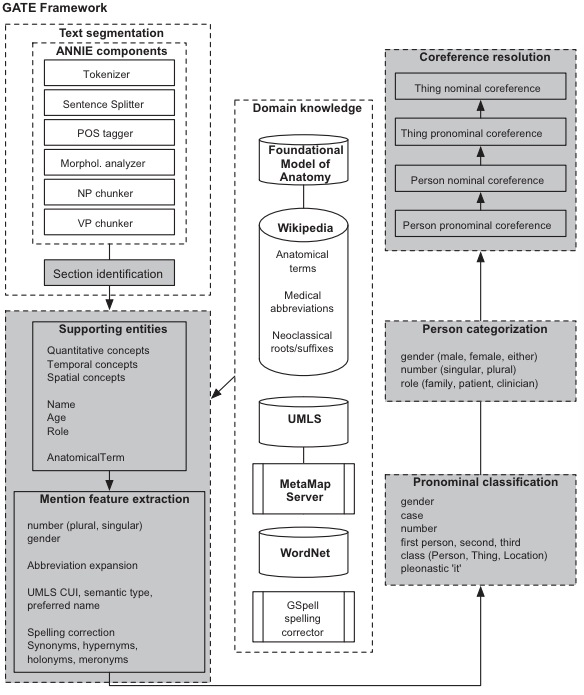
\includegraphics[height=50em]{system.jpg}
  %\end{multicols}
\end{center}

\section{Integrating existing natural language processing tools
for medication extraction from discharge summaries, JAMIA, 2012}
\label{sec:intro} 
\begin{itemize}
\item To develop an automated system to extract
medications and related information from discharge
summaries as part of the 2009 i2b2 natural language
processing (NLP) challenge. This task required accurate
recognition of medication name, dosage, mode,
frequency, duration, and reason for drug administration.
\item 
\end{itemize}

\section{Mining free-text medical records, Pro AMIA Symp, 2001}
\label{sec:intro} 
LifeCode use NLP to extract from a free-text clinical notes:
\begin{itemize}
\item patient demograhics, cheif complaint, illness history, medical history of patient and parents.
\item social history(tobacco,alcohol,drugs,living aggrangement), the nature and extent of the examincation performed by phys.
\item the nature and extent of old records consulted, professonal consultation and medical tests.
\item final diagnoses. potentially also including possbile and ruled-out diagnoses. 
\item the course of treatment including surgical procedures, drug therapy, and monitoring levels. 
\item the serverity of the patinet's condition interms of the phys's stated conclusions and as measured by co-morbidities and the nature and course of treatment.
\item the disposition of the patient at the end of the clinical encounter with the physician.
\end{itemize}
Use domain knowledge to determin
\begin{itemize}
\item the most specific version of each diagnosis and procedure
\item the risk to the patient presented by the medical condition and treatment.
\item the complexity of the medical decision making for the phys.
\item the level of service provided by the physician and the information can be directly reported and that may require validation.
\end{itemize}

\section{Approaches to Text Mining for Clinical Medical Records,
Proceedings of the 2006 ACM symposium on Applied computing, 2006}
\label{sec:intro} 
\begin{itemize}
\item describe a MEDical Information Extraction (MedIE) system 
that extracts and mines a variety of patient information with 
breast complaints from free-text clinical record
\item identify synonyms using UMLS 
(e.g. high blood pressure is a synonym of hypertension) of these 
predefined diseases. This task is simply completed by lookup of 
synonyms in ontology 
\item Graph-based Relation Extraction 
The relation extraction refers to a task that finds pairs of two 
terms in text (usually in a sentence or a couple of consecutive 
sentences) that are semantically or syntactically related to each 
other. Most information extraction (IE) tasks in this project are 
relation extraction or could be transformed to relation extraction 
problem. One type of information for extraction is numeric 
attribute, such as blood pressure, pulse, age and weight of a 
patient. We propose a graph-based approach for  the  extraction  of 
syntactic relation based on the linkage information produced by
Link Grammar Parser [14]. Link Grammar is an original sentence 
parser, producing not only a constituent tree as most parsers yield, 
but  also  a linkage diagram that  consists of links between two 
words. Example: “Blood pressure is 144/90, pulse of 84, temperature of 98.3, 
and weight of 154 pound.”
\item Decision Trees Based Text Classification\\
“She quit smoking five years ago” (former)
“She is currently a smoker” (current)
“None” (never)
“She has never smoked” (never)
\end{itemize}

%----------------------------------------------------------%

\end{document}

